\documentclass{siamart1116}
\usepackage{amsmath, amssymb}
%\usepackage{amsmath,amssymb,amsfonts,graphicx,amsthm,dsfont}
%\usepackage{listings}
%\usepackage{courier}
\usepackage{enumerate}
%\usepackage{color}
%\usepackage[usenames,dvipsnames]{xcolor}
%\usepackage{hyperref,tikz,mdframed}
%\hypersetup{colorlinks=true,urlcolor=MidnightBlue,citecolor=PineGreen,linkcolor=BrickRed}

% \lstset{
% 	basicstyle=\small\ttfamily,
% 	keywordstyle=\color{blue},
% 	language=python,
% 	xleftmargin=16pt,
% }
\usepackage{algorithmicx}
\usepackage{algpseudocode}% http://ctan.org/pkg/algorithmicx
\usepackage{multicol}

\textwidth=5.8in
\textheight=9in
\topmargin=-0.5in
\headheight=0in
\headsep=.5in
\hoffset  -.4in
\pagestyle{empty}

\newcommand{\Fp}{\mathbb{F}_p}
\newcommand{\Q}{\mathbb{Q}}
\newcommand{\Z}{\mathbb{Z}}
\newcommand{\kron}[2]{\left(\frac{#1}{#2}\right)}
\newcommand{\Aut}{\mathrm{Aut}}
\newcommand{\End}{\mathrm{End}}
\newcommand{\SO}{\mathrm{SO}}
\newcommand{\SU}{\mathrm{SU}}
\newcommand{\tr}{\operatorname{tr}}
\newcommand{\dee}{\mathrm{d}}
\newcommand{\deee}{\textbf{\text{\emph{d}}}}

\newcommand{\md}[1]{\textcolor{cyan}{#1}}

\newcommand{\TheAuthors}{V. Chen}

%\newtheorem{theorem}{Theorem}
%\newtheorem{definition}{Definition}

\graphicspath{ {graphics/} }

\title{Comparing hierarchical methods}
\author{\TheAuthors}
\date{}
\begin{document}
\maketitle
\setlength{\unitlength}{1in}
\setlength{\parindent}{0in}
\section{Introduction}
Inspired by the experiment comparing the different clustering algorithms given in \cite{BeLuStZy17}, we ran a similar set of experiments to determine if a hierarchical approach was beneficial to clustering. The clustering algorithms we want to compare are: Fiedler thresholding, nonhierarchical pCN, and two hierarchical algorithms for learning $\tau,\alpha$ as well as the classifying function $u$.
For each of the four algorithms tested, 50 random realizations of the two moons data set were generated with $r=1,N=2000,d=100,$ and varying $\sigma$. We used the same RNG seed for the trials across different algorithms so that these 50 realizations are consistent over the different algorithms tested. With each two moons realization, we tested the classification accuracy with varying fidelity percents for the labeled data. Again, the chosen labeled set $Z'$ is consistent across the trials for different algorithms. Our results are summarized in \cref{fig:compare_hier}.

\begin{figure}[!htb]
\label{fig:compare_hier}
\caption{Classification accuracy of different algorithms for two moons dataset compared with $\sigma$ and percent fidelity. Plotted is the median classification accuracy with error bars that indicate the 25 and 75-th quantiles over the 50 trials for each parameter combination. For the pCN and hierarchical algorithms, we used spectral projection up to the first 50 eigenvectors. We ran 100000 iterations with a burn-in period of 1000, and we fixed $\gamma = 0.1$.}
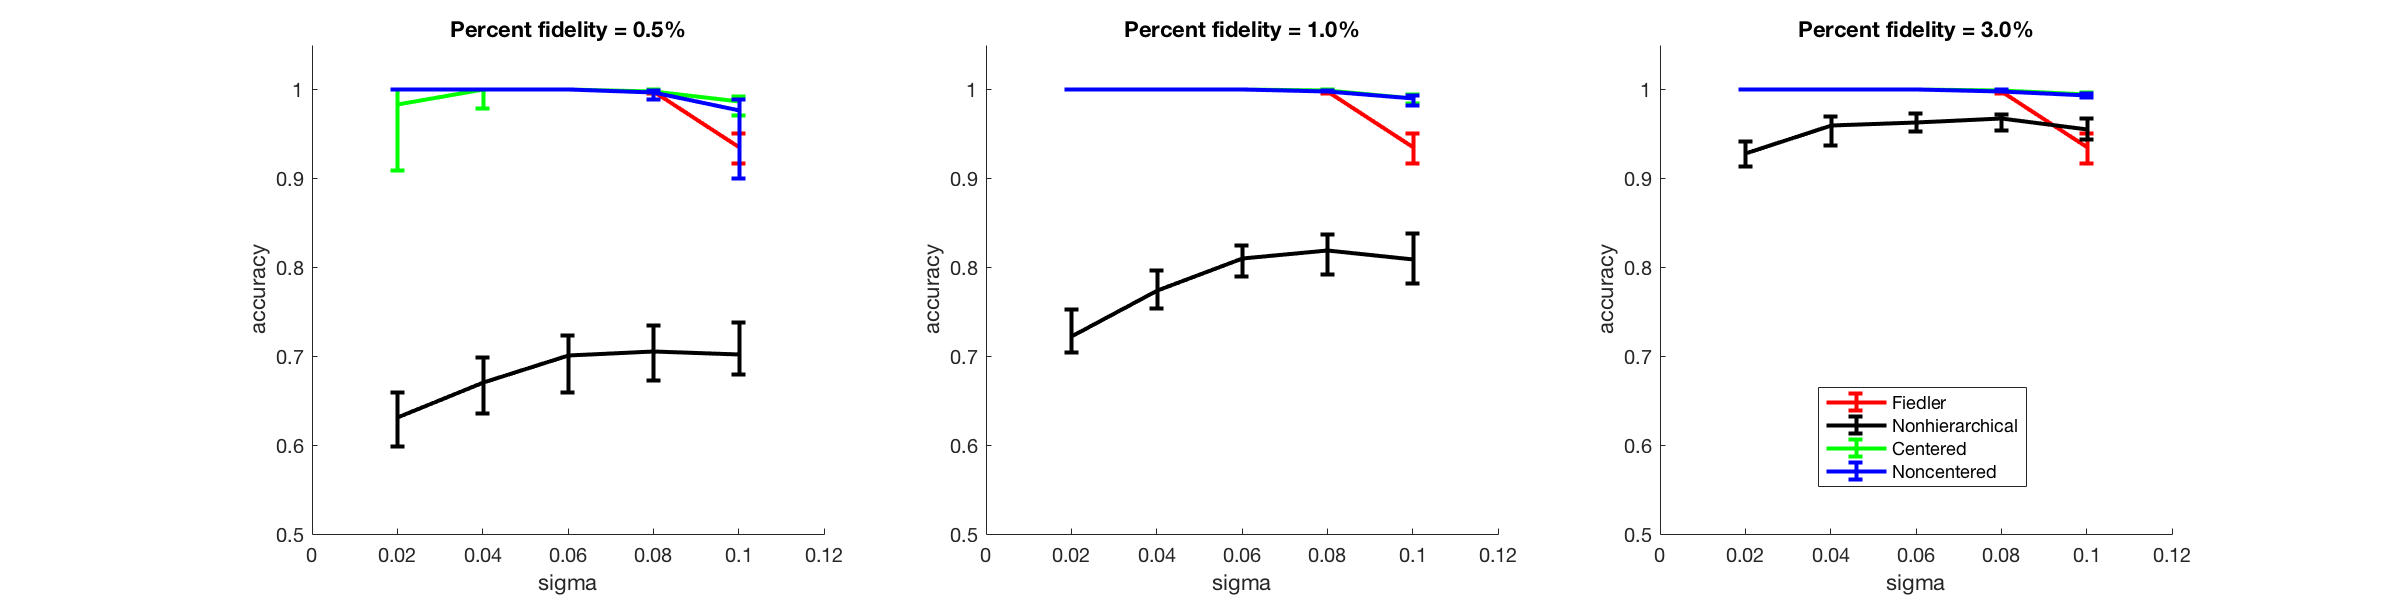
\includegraphics[width=\linewidth]{summary.png}
\end{figure}

\section{Learning $\tau$ and $\alpha$}
In these experiments, the hierarchical algorithms performed much better in classifying the two moons dataset than the nonhierarchical algorithm. We fixed $\tau=\alpha=1$ in the nonhierarchical pCN, while we set $\tau^{(0)}=\alpha^{(0)} = 1$ for the hierarchical algorithms. In the hierarchical algorithms, e allowed $\tau \in [0.01,60]$ and $\alpha \in [0.1,60]$ as the uniform priors.
\begin{figure}[!htb]
\label{fig:compare_alpha}
\caption{Average values of $\alpha$ from the MCMC. Plotted is the median of the averages of $\alpha$ with error bars that indicate the 25 and 75-th quantiles over the 50 trials for each parameter combination. Notice that $\alpha$ is on average much larger in the hierarchical algorithms.}
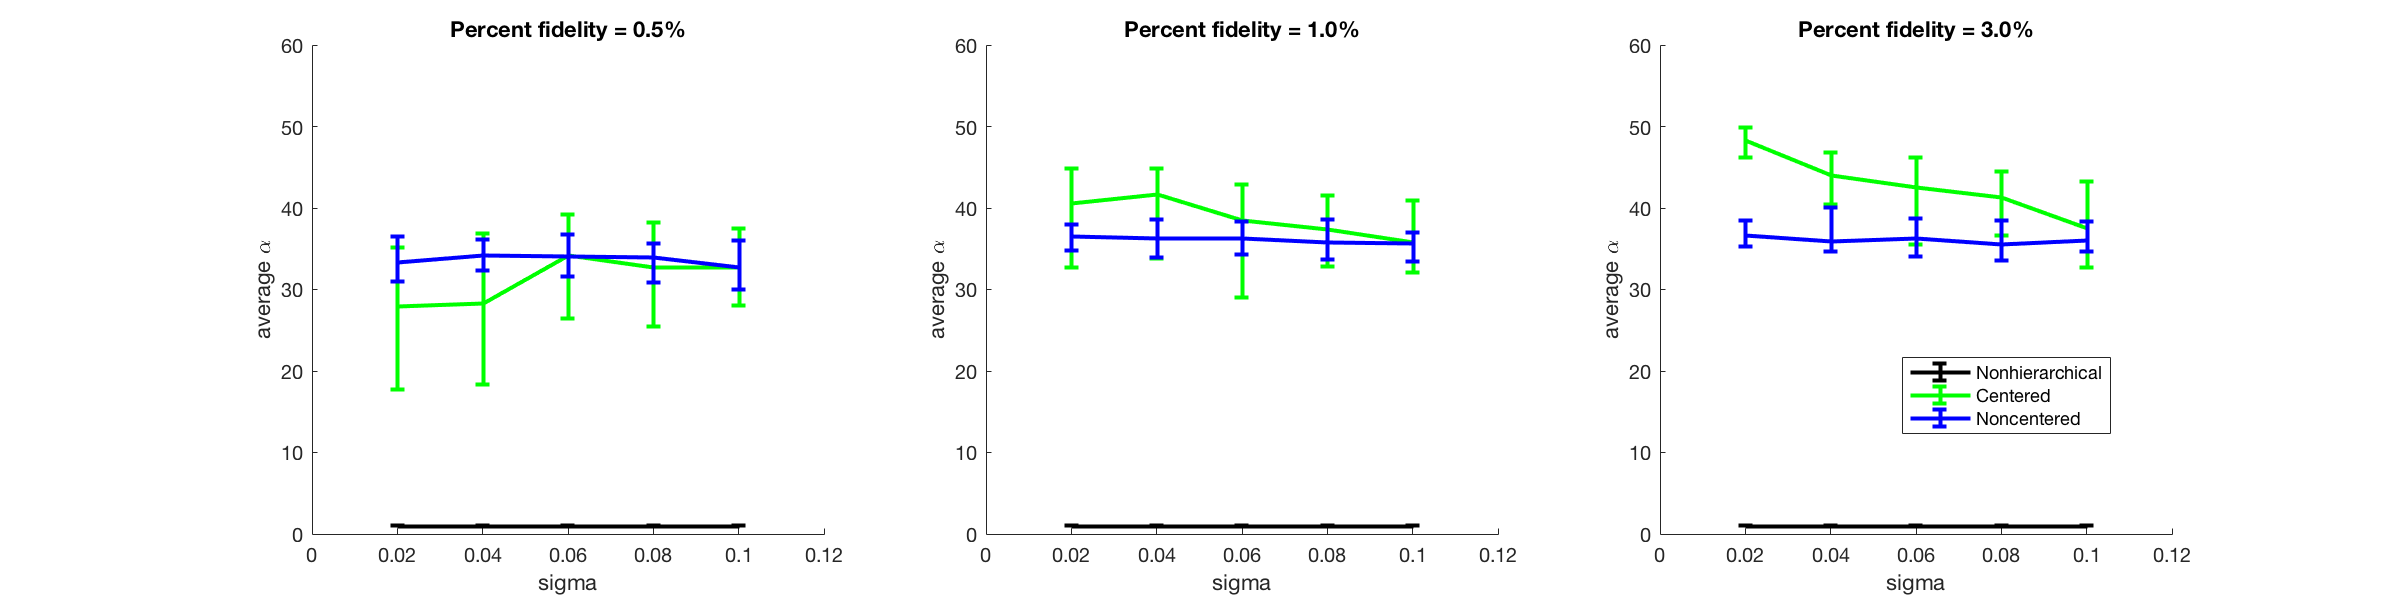
\includegraphics[width=\linewidth]{alpha_averages.png}
\end{figure}

It appears that fixing $\alpha = 1$ in the nonhierarchical algorithm is partially responsible for the discrepancy in performance. With small $\alpha$, the prior on $u$ drops off more slowly with the higher eigenvectors, while larger $\alpha$ enforces that these higher eigenvectors have less influence on $u$. This suggests that for the two moons data set, information for binary classification is concentrated in the lower eigenvectors, as expected.

\bibliographystyle{siamplain}
\bibliography{references}
\end{document}